\documentclass[12pt, letterpaper]{article}

% Packages
\usepackage[utf8]{inputenc}
\usepackage[sorting=none]{biblatex}
\usepackage{amsmath}
\usepackage{tabularx}
\usepackage{graphicx}
\usepackage{csquotes}
\usepackage{float}
\usepackage[normalem]{ulem}
\usepackage{subcaption}
\usepackage{authblk}

% Parragraph formatting
\setlength{\parskip}{1em}

\title{Implementación de un Chatbot utilizando una Red Neuronal Seq2Seq}

\author[1]{Nathaniel Calderón González}
\author[2]{Ernesto Mancebo Tavárez}
\affil[1]{MULCIA, Universidad de Sevilla, Sevilla, España}

\date{Junio 2020}

\begin{document}
    \begin{titlepage}
        \maketitle
        \begin{abstract}
            A continuación se presenta la memoria de un estudio de la implementación de un chatbot mediante el uso de una Red Neuronal bajo la arquitectura Seq2Seq, la misma es entrenada utilizando el Corpus de mensajes del microblog Twitter.
        \end{abstract}
    \end{titlepage}

    \section{Objeto de Estudio}
    \section{Estado del Arte}
    \begin{table}[htb]
        \centering
        \resizebox{\textwidth}{!}{
            \begin{tabular}{l|p{0.4\textwidth}|p{0.7\textwidth}}
                \hline
                \textbf{Implementación} & \textbf{Ventajas} & \textbf{Desventajas} \\
                \hline
                K-Nearest Neightbor & Puede determinar anomalías y fácil de implementar. & Alto consumo de recursos. \\
                Redes Neuronales Artificiales & Aprende patrones de transacciones previas y detecta fraudes en tiempo real. & Se debe de estudiar la técnica a utilizar. \\
                Arboles de Desición & Maneja patrones no lineales. & Igual que las RNA, existen varias técnicas por lo que hay que estudiar cuál conviene. \\
                Outlier Detection Method & Consume menos recursos que otras técnicas y puede trabajar con data en línea (online) & No es tan preciso como otros métodos. \\
                Aprendizaje Profundo & Estudia y extrae patrones de grandes conjuntos de datos. & Es utilizado mayormente en procesamiento de imágenes y del lenguaje, por lo que para este campo hay poca información. \\
                \hline
            \end{tabular}
        }
        \caption{Estado del arte para implementaciones de Chatbots.}
    \end{table}

    \section{Redes Seq2Seq}
    \subsection{Redes Recurrentes - RNN}
    A medida que se analizan estructuras tales como una fotografía, todo el contenido es capturado a la vez y el mismo no cambia a través del tiempo mas no toda la información es analizada de esta manera; existen estructuras donde se depende de la evolución de la misma para conocer su significancia, es decir, se necesita conocer en un determinado punto sus valores previos, es por ello que necesitamos herramientas que traten la información de manera secuencial [Cita Naranjo].

    Para solventar esto se tienen las Redes Neuronales Recurrentes (RNN) las cuales son diseñadas para el análisis de secuencias. Estas redes se caracterizan por lo siguiente:
    
    \begin{itemize}
        \item Comparten parámetros.
        \item Capaces de procesar secuencias de distintas longitudes.
        \item Detectan información relevante que pueden aparecer en distintas posiciones de la secuencia.
    \end{itemize}
    A modo de ejemplificar la última característica de estas redes se tiene \emph{"El 23 de Enero salí a pasear"} o \emph{"Salí a pasear el 23 de Enero"}. 

    Las RNN no conocen el significado de los símbolos que procesan, éstas infieren en el significado a partir de la extructura de la secuencia y la posición de los símbolos. Por otro lado, una RNN es capáz de lograr todo lo mencionado por el hecho de que tales redes tienen un estado al que en ocasiones se le puede escuchar referir como \emph{memoria}.

    El estado o memoria de tal red se logra a partir del hecho de que una RNN son redes con bucles dentro de ella.

    \begin{figure}[H]
        \centering
        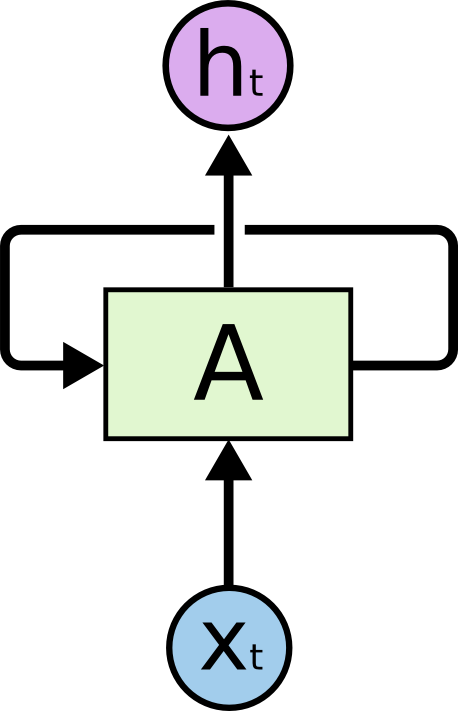
\includegraphics[width=\linewidth]{img/RNN-rolled.png}
        \caption{Ilustración de una RNN.}
    \end{figure}

    En la representación se tiene un trozo de red $A$ la cual toma como entrada un $x_t$ y emite un valor $h_t$, de este modo, utilizando el bucle mencionado, la información pasa al siguiente paso dentro de la red. Dicho ya esto, podemos ilustrar una red recurrente como una red con múltiples copias de sí misma.
    [Understanding LSTMs]

    \begin{figure}[H]
        \centering
        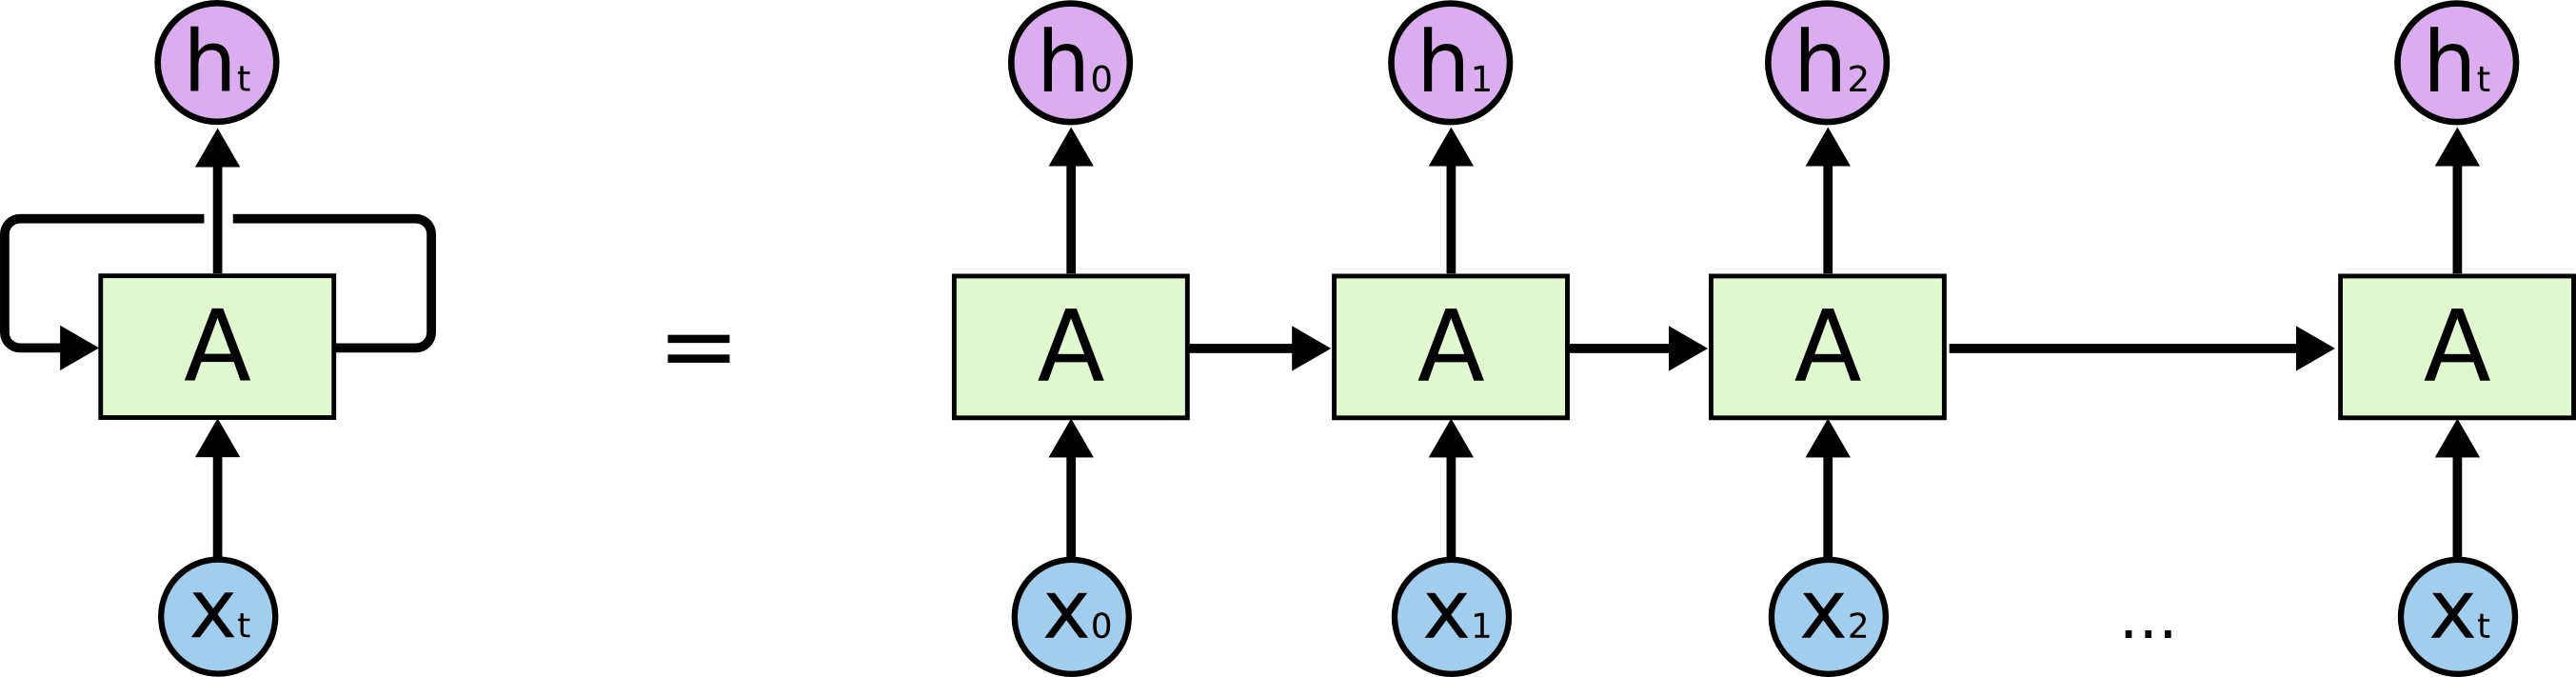
\includegraphics[width=\linewidth]{img/RNN-unrolled.png}
        \caption{Ilustración de la evolución de una RNN a través del tiempo $t$.}
    \end{figure}
    
    Este comportamiento en secuencia es lo que enlaza las RNN con secuencias y listas, por ellos, tales redes son exitosas para problemas de reconocimiento de voz, modelado del lenguaje, traducción, contextualización de imágenes y otras aplicaciones relacionadas.
    [RNN Andej]

    \subsection{Redes Long Short-Term Memory - LSTM}
    Una variante las RNN capáz de aprender a partir de dependencias a largo plazo es la Long Short Term Memory, muchas veces llamadas tan solo LSTM.
    
    Las LSTM fueron diseñadas con la intención de evitar problemas de dependencia a largo plazo, con la naturaleza de recordar información por un largo período de tiempo.
    
    La estructura interna de una LSTM varía un poco de una RNN regular, donde en vez de tener una única capa, tiene cuatro y cada una interactúa de un modo distinto.

        \begin{figure}[H]
            \centering
            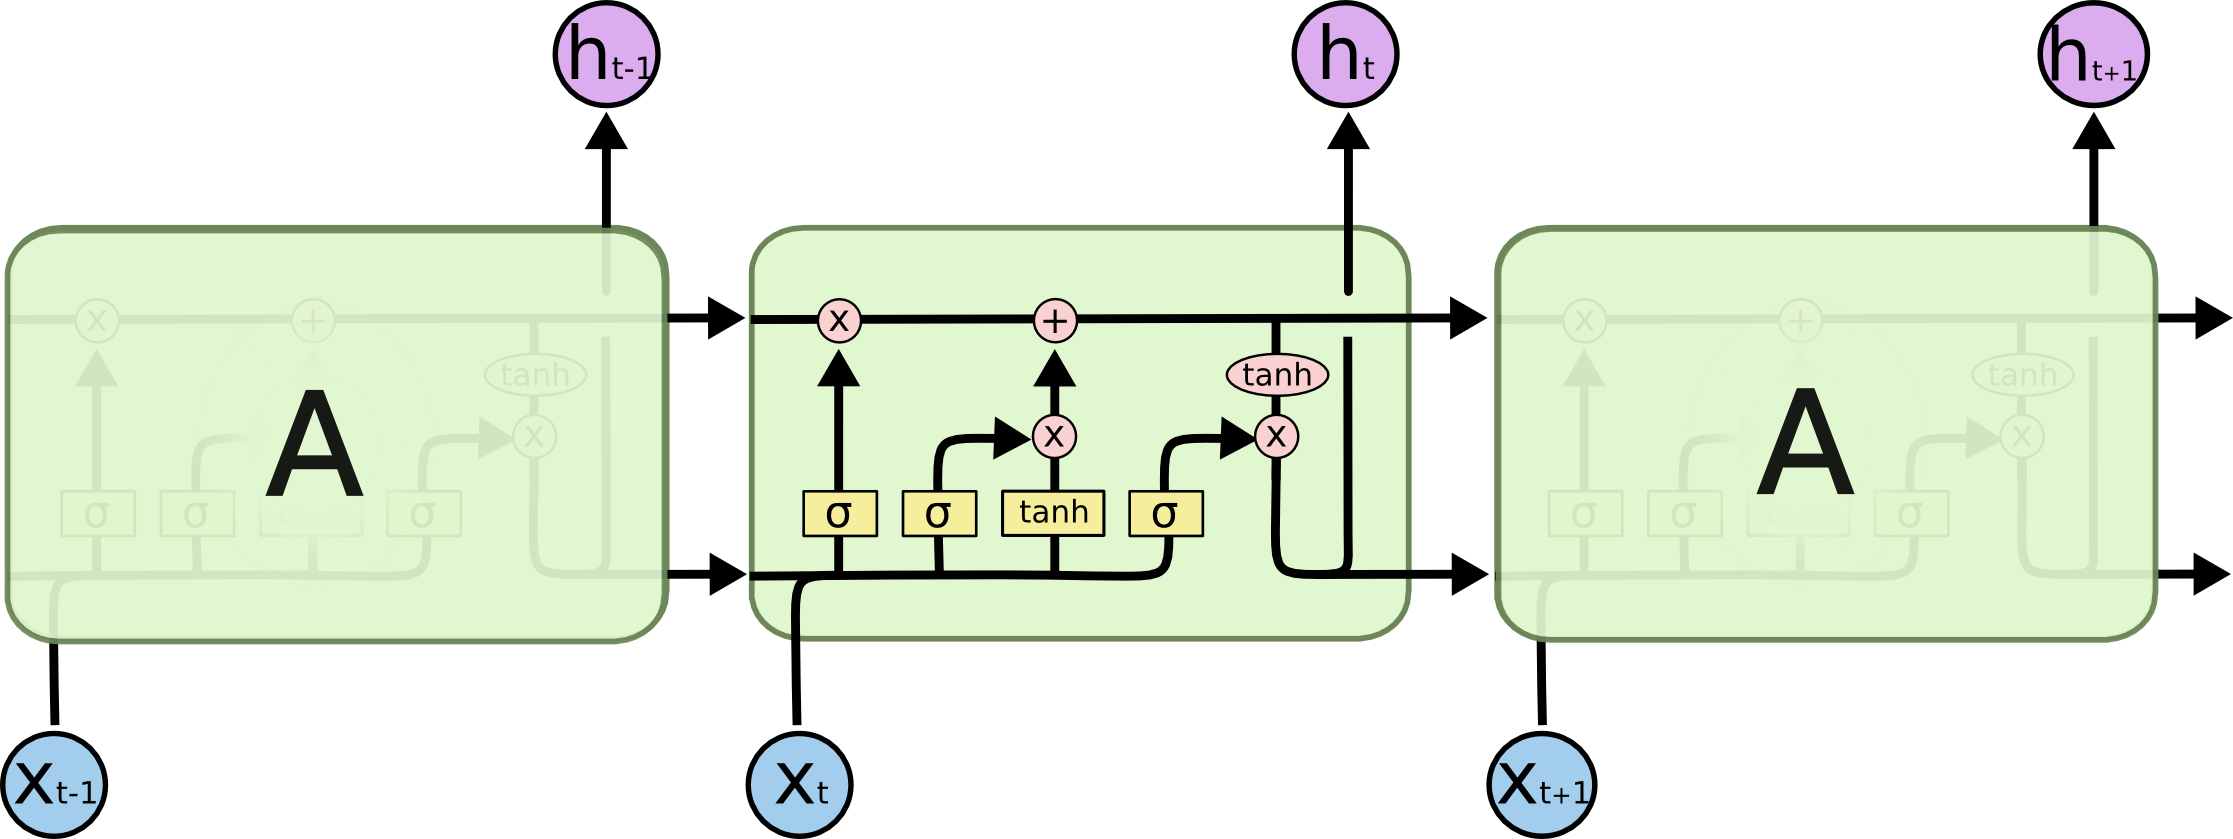
\includegraphics[width=\linewidth]{img/LSTM3-chain.png}
            \caption{Ilustración de una red LSTM.}
        \end{figure}

        A continuación tenemos una radiografía de lo que conforma una red LSTM.
        \begin{figure}[H]
            \centering
            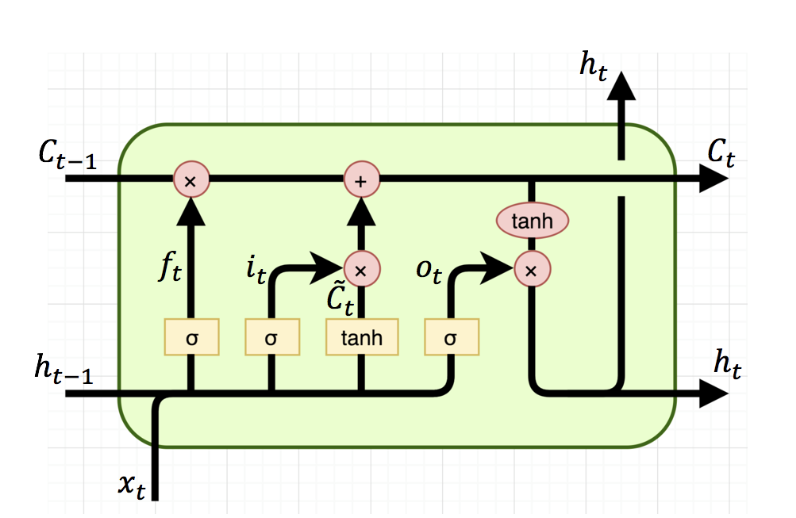
\includegraphics[width=\linewidth]{img/LSTM3-cell-A.png}
            \caption{Composición interna de una LSTM.}
        \end{figure}

        Definiendo cada elemento de la celda de la siguiente manera:
        $
            \begin{aligned}
            f_t  & = \sigma(W_f\dot{\[h_{t-1},x_t\]} + b_f) \\
            i_t & = \sigma(W_i\dot{\[h_{t-1}, x_t\]} + b_i) \\
            \tilde{C}_t & = \text{tanh}(W_c\dot{\[h_{t-1}, x_t\]} +b_C) \\
            o_t & = \sigma(W_o\dot{\[h_{t-1}, x_t\]} + b_o) \\
            h_t & =  o_t*\text{tanh}(C_t)
            \end{aligned}
        $
        Donde decimos que:
        \begin{itemize}
            \item $W$ representa las matrices de pesos de la red.
            \item $x_t$ representa el vector de entrada en un tiempo t
            \item $h_{t-1}$ representa el vector de salida producido en la computación previa.
            \item $C_{t-1}$ representa la celda estado(por algunos llamado memoria) producida en la computación previa.
            \item $b$ representa el conjunto de sesgos o \emph{bias}.
            \item $\sigma$ epresenta la función de activación Sigmoide o Sigmoid(en inglés), la cual consiste en transformar el valor de entrada en una escala de 0.0 a 1.0, los valores mayores de 1.0 son transformados a 1.0 y viceversa.
            \item \emph{tanh} epresenta la función de activación Tangente Hiperbólica o tanh, en cambio esta consiste en transformar el valor de entrada en una escala entre -1.0 y 1.0. Se dice que para muchos casos esta función permite conseguir un mejor rendimiento y es más fácil de entrenar, que la función sigmoide.
            \item La celda $C$ aprende a memorizar información basado en conexiones recursivas entre celdas.
            \item $i$ representa la compuerta de entrada utilizada para controlar el flujo de error de las $C$ celdas de estado de entrada(inputs cell state), y así evitar los problema con los pesos de entrada que ocurre en las RNN tradicionales, donde el mismo peso es utilizado para decidir qué información de entrada retener y cuál descartar.
            \item $o$ representa la compuerta de salida que controla el flujo de error de las celdas de estado de salida(outputs cell state) c, por la misma razón para evitar los problemas que ocurren en las RNN tradicionales.
            \item $i$ permite a la red decidir cuándo escribir información en c, y ocuándo leer información desde c, ambas representan lo que podemos denominar como bloque de memoria de la red LSTM.
            \item $f$ es una compuerta de olvido utilizada para limpiar la memoria y ayuda a la red a modelar secuencias continuas.
        \end{itemize}
.




    [Understanding LSTMs]
    \subsection{Redes Seq2Seq}
    [Chatbot]

    \section{Corpus}
    \section{Implementación}

    \section{Resultados}
    \section{Conclusiones}

    \pagebreak
    % \printbibliography[title={Bibliografía}]
\end{document}